\documentclass[letterpaper]{article}

%% Language and font encodings
\usepackage[english]{babel}
\usepackage[utf8x]{inputenc}
\usepackage[T1]{fontenc}

%% Sets page size and margins
\usepackage[letterpaper,margin=1in]{geometry}

%% Useful packages
\usepackage{amsmath}
\usepackage{graphicx}
\usepackage[colorinlistoftodos]{todonotes}
\usepackage[colorlinks=true, allcolors=blue]{hyperref}
\usepackage{graphicx}
\usepackage{subcaption}
\usepackage{float}
\usepackage{algorithm}
\usepackage[noend]{algpseudocode}
\usepackage[autostyle]{csquotes} 
\usepackage[title]{appendix}


\makeatletter
\def\BState{\State\hskip-\ALG@thistlm}
\makeatother

\title{Improving Sepsis Treatment using Mixture-of-experts}
\author{Peng, Xuefeng\\
		\texttt{xpeng@g.harvard.edu}
        \and
        Ding, Yi\\
        \texttt{yid095@mail.harvard.edu}
        \and 
        Wihl, David\\
        \texttt{davidwihl@g.harvard.edu}
        }
\date{December 14, 2017}
\begin{document}
\maketitle

\begin{abstract}
Sepsis is main cause of mortality in the ICU and the most expensive treatment in hospitals. Patients with different physiological states respond to medical treatments very differently, and this makes sepsis management a worldwide challenge. Therefore, treatment tailored to individual patient provides significant value. In this paper, we propose a mixture-of-experts framework to further individualize sepsis treatment for each step in a patient's clinical course. The mixture model consists of kernel and DQN experts, utilizing two different gating strategies to switch actions between policies suggested from both experts: a conventional logit-based gate as well as a novel reinforcement learning based gate. Our experiments indicates that the mixture-of-experts model outperforms both kernel and DQN experts, and is thus promising for improvement in sepsis treatment. In order to reduce variance of the suggested actions, we constrain by commonly observed physician interventions. The mixed policy, including accounting for
physician actions, yields a projected significant decrease in patient mortality with certain caveats. 

\end{abstract}

\section{Introduction}

Sepsis is considered a medical emergency that requires rapid treatment. Each year, it not only costs hospitals billions of dollars but also causes tremendous patient mortalities. Individual patient respond to medical treatments very differently, and this makes sepsis management extremely challenging. Physicians have no uniform agreement on sepsis management; however, among various treatments, there are two drugs that are widely used to care for septic patients: intravenous (IV) fluid (adjusted for fluid tonicity) and vasopressor (VP). These two drugs are used to correct the hypovolemia, and counteract sepsis-induced vasodilation, respectively. Treatment decisions are critical, as they lead to extreme variation on patient mortality \cite{waechter2014interaction}, thus, individualized treatment has a potential to improve the sepsis management.

In this work, we propose a mixture-of-experts framework aiming to tailor treatment for patients. The mixture-of-experts framework contains kernel and DQN experts using a gating strategy to switch action between policies suggested from both experts. For kernel expert, we train a recurrent auto-encoder to encode all of a patient's physiological observations during the stay in the ICU. Given a new patient, the  observations are encoded to search for the nearest neighbors, which is used to derive a neighbor-based policy maximizing the survival rate. With respect to the DQN expert, we first encode patient observations into continuous state representation recurrently. Thus, the information from previous states are preserved in the current state. Then, we train the DQN using these representations. At each given state, the DQN agent takes an action with the highest Q-value, given the ultimate goal of improving the overall survival rate. We attempted two approaches to combine the policies produced from both experts. The first one, we call logistic-based switching, uses pre-trained logits to decide a probability distribution over actions from two experts, and subsequently the action with higher probability will be selected. We use WDR (weighted doubly robust) \cite{thomas2016data} as the unbiased off-policy estimator to evaluate the policy derived from kernel, DQN, and the mixture-of-experts. The mixture-of-experts outperforms each separate expert in the testing set. The second, which we call RL-based gating, chooses the action by searching through the state-action space to find the set of actions leading to the lowest mortality. 

In particular, our contributions can be summarized as below:

\begin{itemize}
\item We used recurrent auto-encoder to encode patient ICU physiological states so that the interaction between these states are taken into consideration.
\item We trained kernel and DQN experts to learn policies which maximize the patient survival rate. 
\item We created a mixture-of-experts framework that can switching actions between kernel and DQN experts to further improve the treatment for patient at any given time step.
\item We created an RL-based mixture-of-experts that choses the best action between physician, kernel and DQN
experts to discover the path to the lowest mortality.
\end{itemize}

\section{Related Work}

This work builds heavily on the prior work of Raghu, Komorowski et al. \cite{DBLP:journals/corr/RaghuKCSG17}
in terms of using a Dueling Double-Deep Q Network (Dueling DDQN), discretized patient states and 
discretized physician actions for administering fluids and vasopressors.  Combining kernel
and reinforcement learning experts uses some of the methods applied by Parbhoo, Bogojeska, et al. 
\cite{parbhoo2017combining} in the HIV patient treatment context.

\section{Data and Preprocessing}

\subsection{Dataset}
We employ the same patient data used in \cite{DBLP:journals/corr/RaghuKCSG17}. The patient data is obtained from Multiparameter Intelligent Monitoring in IntensiveCare (MIMIC-III v1.4) database \cite{johnson2016mimic}. The dataset consists of patient from different age groups and genders with various physiological attributes. Each patient's total ICU stay is partitioned into one or more 4-hour windows, and each window counts as a set of observations. Observations describes a patient's condition (e.g. blood pressure, respiratory rate, and sequential organ failure assessment (SOFA) score) as well as the treatments (e.g. iv-fluids, vasopressor and mechanical ventilation) applied during that time window.
%The full list of physiological attribute and treatment terminologies are shown in Appendix \ref{appendix-terminologies}. 

\subsection{Data Cleaning}
The dataset contains observations that are invalid; for instance, the fluids injected to a patient cannot be negative. Therefore, we eliminate patients with invalid observations. Unnecessary attributes such as chart-time, which is used to describe when the patient was moved into ICU, are excluded. 

\subsection{Data Preprocessing}
Physiological attributes and treatment including demographics, lab-values, vital signs, and input/output events have different scales; therefore, we apply preprocessing to normalize. Table \ref{table:preprocessing} describes the attributes and their corresponding preprocessing methods. After the standardization and log transformation, we rescale all values into $0-1$.  

\begin{table}[H]
\centering
\caption{Physiological attributes, treatments and corresponding preprocessing methods}
\label{table:preprocessing}
\begin{tabular}{|l|l|}
\hline
Preprocessing   & Attributes \\ \hline
Standardization & \begin{tabular}[c]
{@{}l@{}}\texttt{age,Weight\_kg,GCS,HR,SysBP,MeanBP,DiaBP,RR,Temp\_C,FiO2\_1,}\\ 
  \texttt{Potassium,Sodium,Chloride,Glucose,Magnesium,Calcium,Hb,}\\ 
  \texttt{WBC\_count,Platelets\_count,PTT,PT,Arterial\_pH,paO2,paCO2,}\\ 
  \texttt{Arterial\_BE,HCO3,Arterial\_lactate,SOFA,SIRS,Shock\_Index,PaO2\_FiO2,}\\ 
  \texttt{cumulated\_balance\_tev, Elixhauser, Albumin, CO2\_mEqL, Ionised\_Ca}
  \end{tabular} \\ 
  \hline
  Log transformation    & \begin{tabular}[c]
    {@{}l@{}}\texttt{max\_dose\_vaso,SpO2,BUN,Creatinine,SGOT,SGPT,Total\_bili,}\\
    \texttt{INR,input\_total\_tev,input\_4hourly\_tev,output\_total,output\_4hourly}
    \end{tabular}                             \\ \hline
\end{tabular}
\end{table}

\subsection{State Clustering and Treatment Discretization}

We use K-means to cluster patients' physiological observations into states. Since we share the same dataset with \cite{DBLP:journals/corr/RaghuKCSG17}, we adopt the same k-value, $k=750$.

Furthermore, \cite{DBLP:journals/corr/RaghuKCSG17} shows that among all those medical interventions, there are two most critical interventions physicians usually take to treat septic patients. They are volume of intravenous (IV) fluid (adjusted for fluid tonicity) and maximum vasopressor (VP) dosage. The dosage given of those two drugs are recorded at each 4-hour window. The dosage for each of them is discretized into 5 bins, resulting in a $5\times5$ action space indexed from 1 to 25. Note that the first action means ``no action'' -- neither IV-fluid nor vasopressor are prescribed.

\subsection{Mortality}

There are two attributes indicating mortality: \texttt{died\_in\_hospital} and \texttt{died\_in\_90\_days}. Our work focuses on using \texttt{died\_in\_hospital} to calculate mortality rate as \texttt{died\_in\_90\_days} introduces extra confounding factors. 
In the dataset, the mortality rate is $12.2\%$ in hospital and approximately $25\%$ after 90 days. We demonstrate the mortality rate in different age group in Figure \ref{fig:mort_by_age}. In general, higher age group associates with a higher mortality rate.

\begin{figure}[H]
\centering
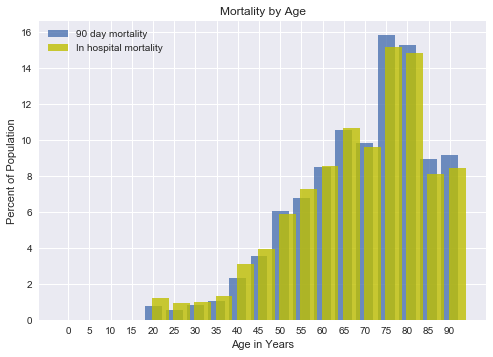
\includegraphics[width=0.6\textwidth]{figures/mort_by_age.png}
\caption{\label{fig:mort_by_age} Mortality rate in different age groups.}
\end{figure}

\subsection{SOFA Score}

In order to evaluate patient stability upon entry to the ICU as well as progression of the clinical
course, we use the sequential organ failure assessment (SOFA) score.
The score is a combination of six different scores, one each for the respiratory, cardiovascular, hepatic, coagulation, renal and neurological systems. Each system is evaluated on a scale of $0-4$
where higher is worse. The per-system score is totaled.
The higher total score indicates higher chance of death.

As seen in figure \ref{fig:SOFA}, the SOFA scores did not change dramatically between the
beginning and end of most patient episodes, leading to motivation that an improved policy may lead to 
improved patient treatment as compared to current practices.

\begin{figure}[H]
  \centering
  \begin{subfigure}{0.4\linewidth}
  \centering
  	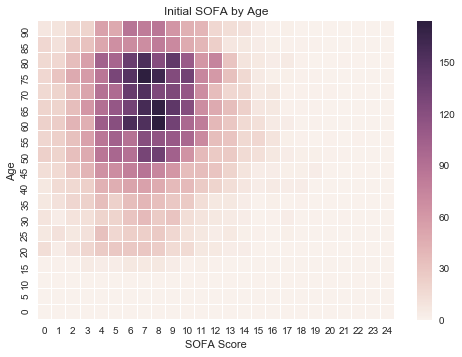
\includegraphics[width=1.0\linewidth]{figures/init_SOFA.png} %\hfill
  	\caption{Initial SOFA scores by age}
  	\label{fig:init_SOFA}
  \end{subfigure}%
  \begin{subfigure}{0.4\linewidth}
  \centering
  	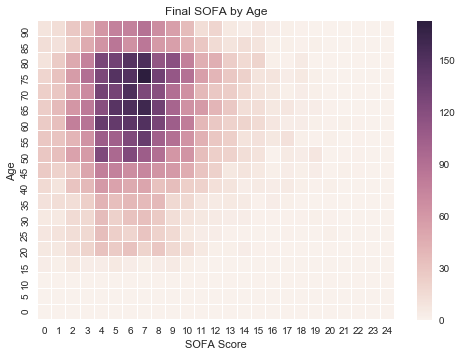
\includegraphics[width=1.0\linewidth]{figures/fin_SOFA.png}\hfill
  	\caption{Final SOFA scores by age}
  	\label{fig:fin_SOFA}
  \end{subfigure}
  \caption{SOFA Scores by Age}
  \label{fig:SOFA}
\end{figure}

\section{Methods}
This section describes the methods used to learn the optimal policy for each expert and gating function. We first use a kernel method to derive group-based policy. 
Since \cite{DBLP:journals/corr/RaghuKCSG17} demonstrates the effectiveness of deep reinforcement learning approach on improving sepsis treatment, we also apply DQN, but in our case, we attempt to maximize the patient survival rate. Finally, our mixture-of-experts model is formed by combining these two methods. In the following subsections, we first describe our kernel method in details; second, we present the DQN method, and then followed by the mixture-of-experts model. 

\subsection{Kernel Expert}

Deriving optimal policy based on a Markov Decision Process (MDP) assumes that each state transition in the patient’s history is independent from all previous states, which may not be true. Therefore, we explored a direct policy learning via kernel. Our first step is transforming patient's set of observations into a single representation vector. The observations in the set are ordered by a 4-hour window since the patient arrived at ICU; thus, one patient's observations are highly temporally correlated. In order to capture this temporal information as much as possible, we applied a recurrent autoencoder. Given a new patient and one or more observations, we encode them into a single representation vector and sought the 500 nearest neighbors using Euclidean distance. Then a policy is learned directly for the given patient based on those neighbors. In summary,

\begin{itemize}
\item Use recurrent auto-encoder to encode each patient’s all current ICU-stay histories into a representation with fixed length.
\item Search 500 nearest neighbors using Euclidean distance.
\item Learn policy for the given new patient that leads to the highest survival rate based on the nearest neighbors.
\end{itemize}

\subsubsection{Recurrent Autoencoder}

The observations collected every 4-hours from a patient in ICU stay are temporally correlated. Therefore, we use recurrent structured LSTM-autoencoder to encode those observations. 

Specifically, our autoencoder utilizes one LSTM layer for both encoder and decoder. The major advantage of this structure is that each time the embedding of the previous observation and the current observation are propagated to the network together, so that the next hidden state contains the information of both current and previous observations. By doing this recurrently, the information from all previous observations can be preserved. The last hidden states from the LSTM network is our final embedding. In order to train the autoencoder, we then repeat the last hidden state $|observations|$ times, and decode them back; and the loss is calculated as MSE between the original observations and the decoded observations. Our final encoder and decoder both contains one LSTM layer, with 128 hidden units. Figure \ref{fig:lstm-autoencoder} demonstrates the model structure.

\begin{figure}
\centering
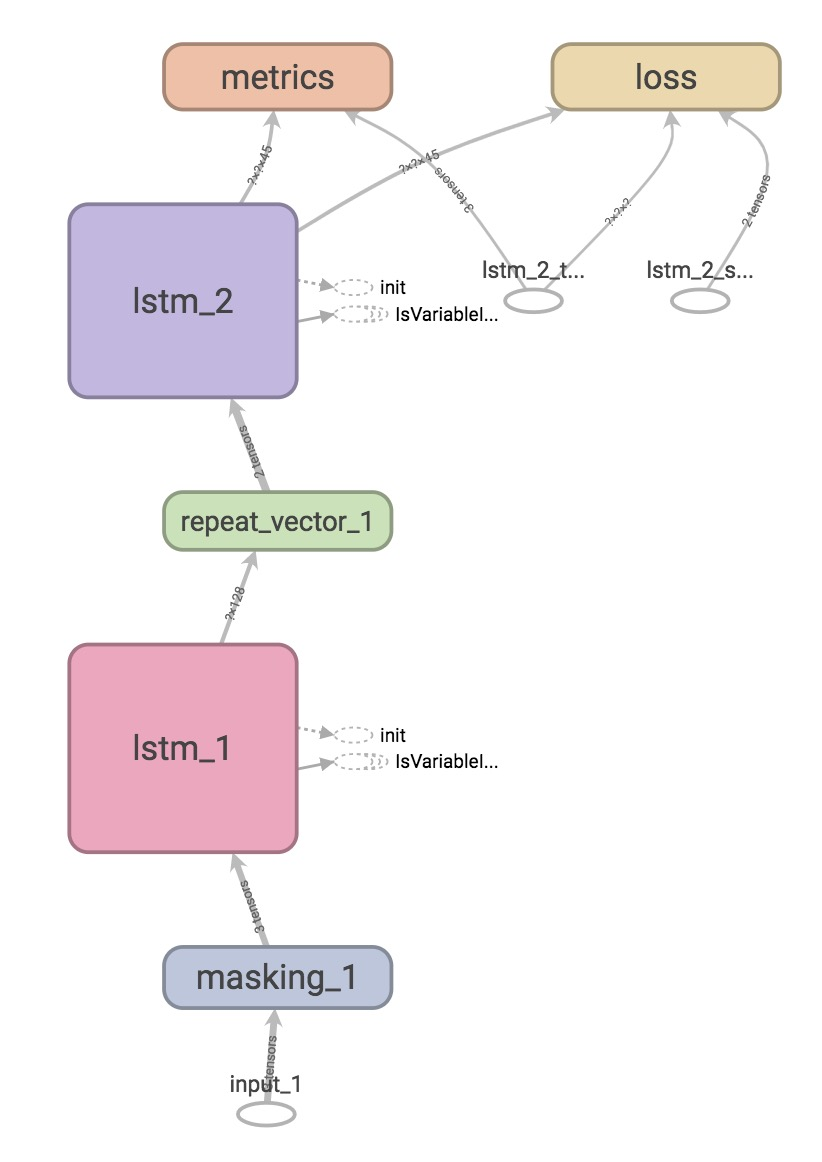
\includegraphics[width=0.4\textwidth]{figures/lstm-autoencoder.jpg}
\caption{\label{fig:lstm-autoencoder}The LSTM-autoencoder model structure. \tiny{Diagram generated from Tensorboard}.}
\end{figure}

We create a feature matrix for each patient, where row $i$ is the observation at timestep $i$. However, some patients have more stays than others; therefore, we find the longest stay, which is 20, and represent every patient to a $20 \times |features|$ matrix. For patients who do not have 20 stays, we pad the empty rows with 0. The padding will be masked when computing the loss.

While training the model, we apply the Adam optimizer to minimize the MSE, and use $R^2$ as the metric. After roughly 100 epochs, the loss on test set is decreased from $4.5\times 10^{-2}$ to $5.0 \times 10^{-3}$; and the $R^2$ score has increased from $0.4$ to $0.92$. The loss and metric are shown in Figure \ref{fig:lstm-train}.

\begin{figure}[H]
  \centering
  \begin{subfigure}{0.5\linewidth}
  \centering
  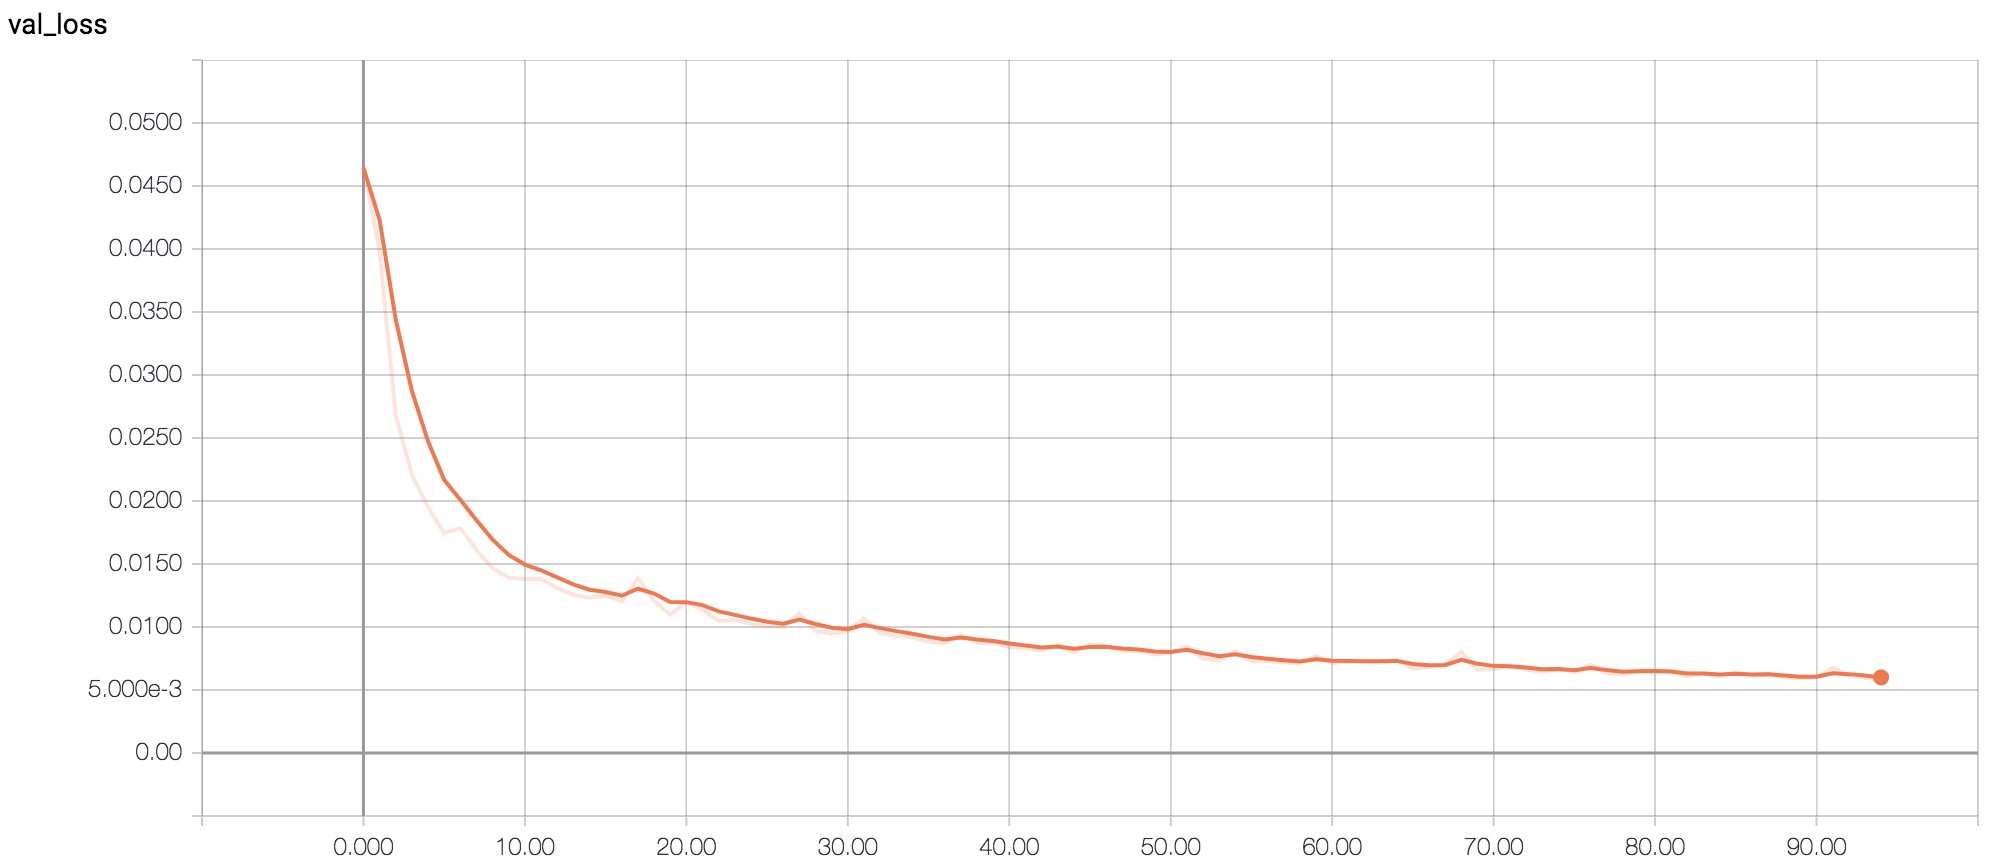
\includegraphics[width=0.9\linewidth]{figures/lstm-loss.jpg}\hfill
  \caption{MSE loss for each epoch}
  \label{fig:lstm-train:a}
  \end{subfigure}%
  \begin{subfigure}{0.5\linewidth}
  \centering
  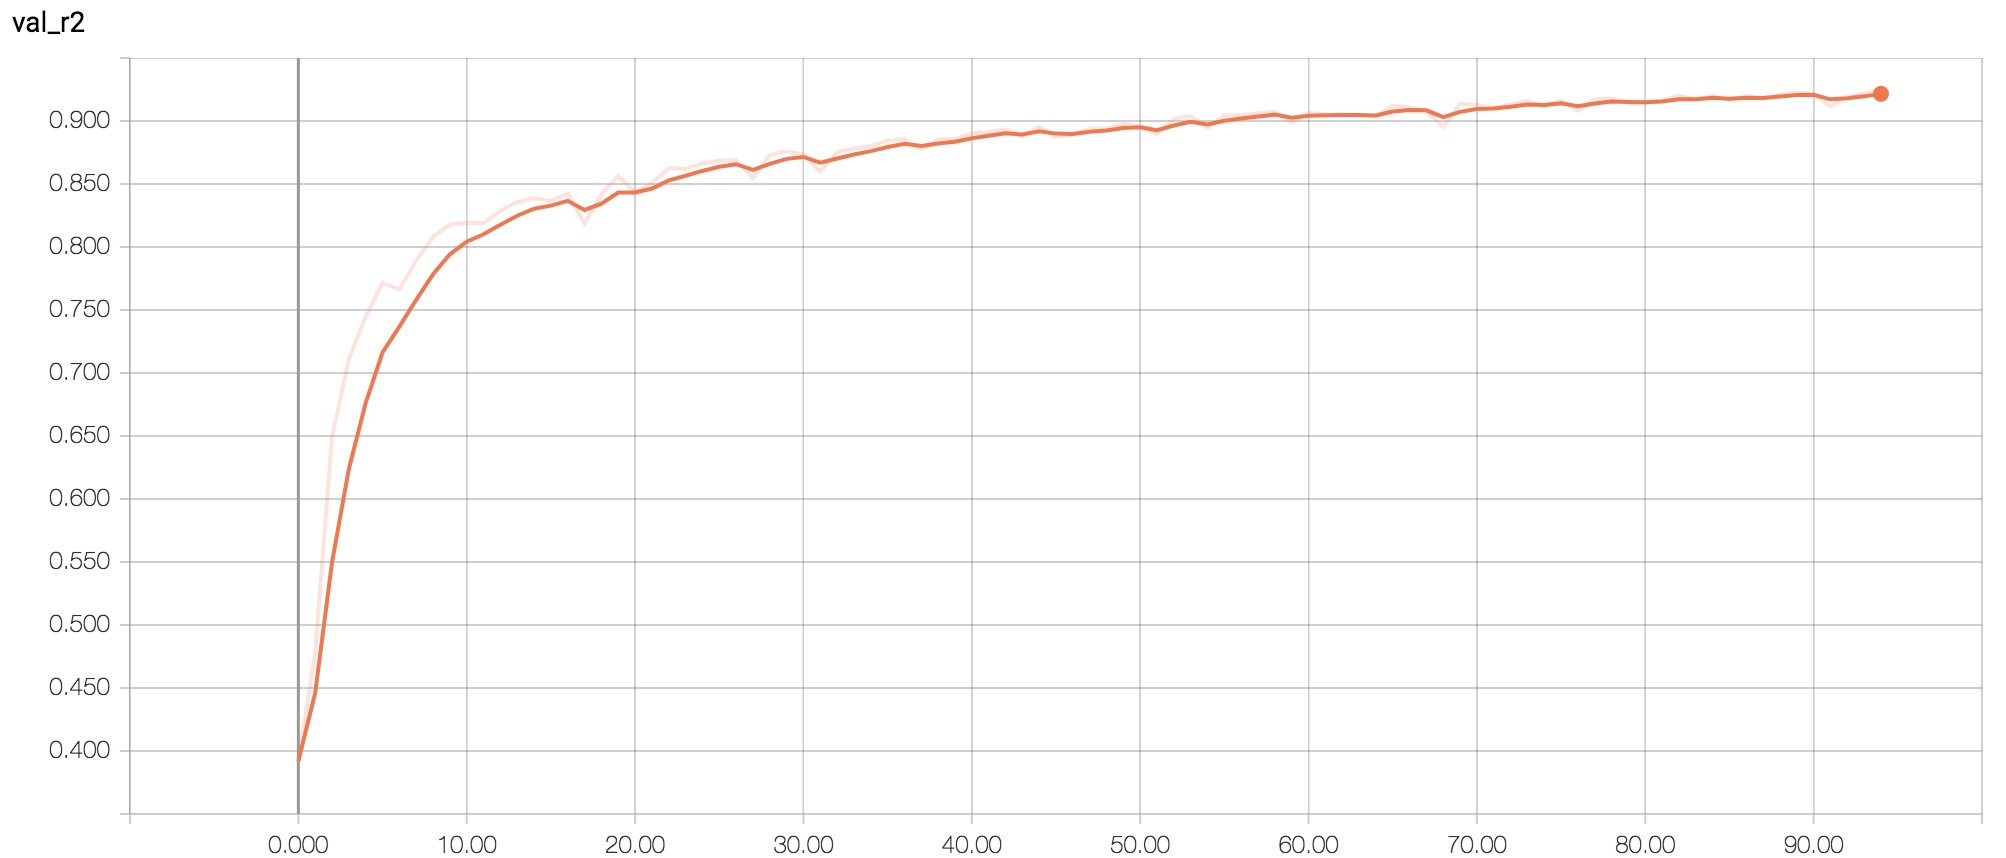
\includegraphics[width=0.9\linewidth]{figures/lstm-r2.jpg}\hfill
  \caption{$R^2$ score for each epoch}
  \label{fig:lstm-train:b}
  \end{subfigure}
  \caption{loss and metrics for training the LSTM-autoencoder}
  \label{fig:lstm-train}
\end{figure}

\subsubsection{Neighbor-based Policy Derivation}
Given arbitrary number ($<20$) of ICU stay observations of a patient, we first encode them into 128-sized representation vector using the LSTM-autoencoder trained above. Then, we find 500 nearest neighbors from training dataset based on the Euclidean distance. The action that gives the highest survival rate among the same discretized state is chosen for the current state of the patient. Figure \ref{fig:kernel_policy} illustrates this process.

\begin{figure}[H]
\centering
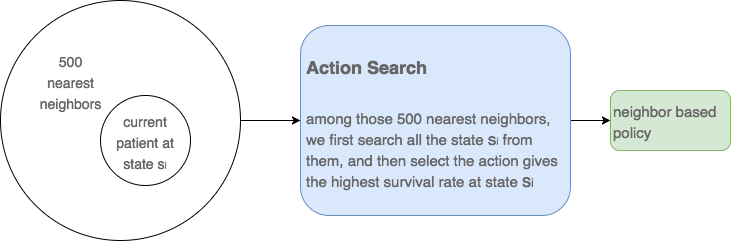
\includegraphics[width=0.7\textwidth]{figures/kernel_policy.png}
\caption{\label{fig:kernel_policy} The process of deriving neighbor-based policy.}
\end{figure}

\subsection{DQN Expert}
Dueling DQN structure has been successfully applied to derive a policy that outperforms the physician policy in \cite{DBLP:journals/corr/RaghuKCSG17}. Therefore, we adopted the DQN structure from it. In order to differentiate the feedback of a treatment caused by a patient's current underlying physical condition, or the treatment itself, we use Dueling Double Deep-Q-Network introduced by \cite{wang2015dueling}. To stabilize the training process and improve the performance, we applied three techniques: 1) reward clipping, 2) reward regularization, 3) and prioritized experience replay. In this section, we refer DQN expert as \textit{agent}.

\subsubsection{Continuous State Representation and Reward Formulation}
\label{section:reward_formulation}

To train the agent, we first treat each observation as a state so that the state space becomes continuous. \cite{DBLP:journals/corr/RaghuKCSG17}'s work uses a sparse autoencoder to encode the observations into a vector of length 200. However, that encoding did not consider the interaction between states. In our work, we use LSTM-autoencoder to encode each state, so that the representation of current state incorporates the information from previous states. 

In terms of reward, for each patient, we issue $0$ reward for states that are not the final state, i.e. the state where the patient is discharged from ICU. In the final state, if the patient is alive we issue a $+15$ reward; otherwise, we issue $-15$.

\subsubsection{Agent Training}

The agent is trained for 200,000 steps (batch size $\ = 32$) with the objective of minimizing the TD-error. At each given state, the agent is trained to take an action with the highest Q-value, in order to achieve the ultimate goal of improving the overall survival rate. Figure \ref{fig:dqn_train} demonstrates the loss and mean Q-values of physician and agent actions for each epoch. The learned policy on test set will be presented in section \ref{section:dqn_policy}.

\begin{figure}[H]
  \centering
  \begin{subfigure}{0.5\linewidth}
  \centering
  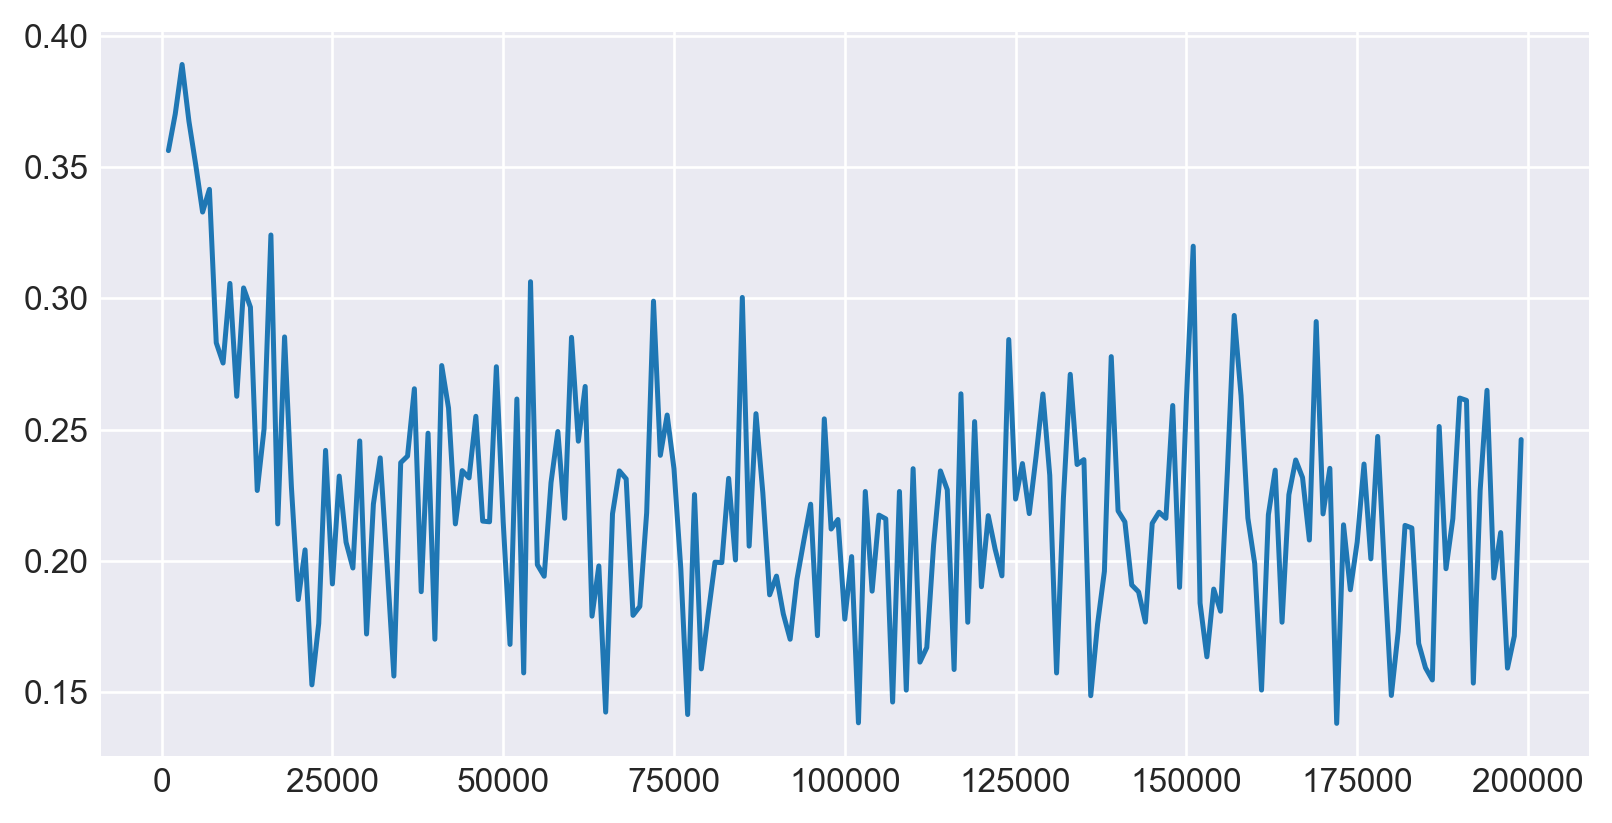
\includegraphics[width=0.9\linewidth]{figures/dqn_loss.png}\hfill
  \caption{The loss for each epoch.}
  \label{fig:dqn_loss}
  \end{subfigure}%
  \begin{subfigure}{0.5\linewidth}
  \centering
  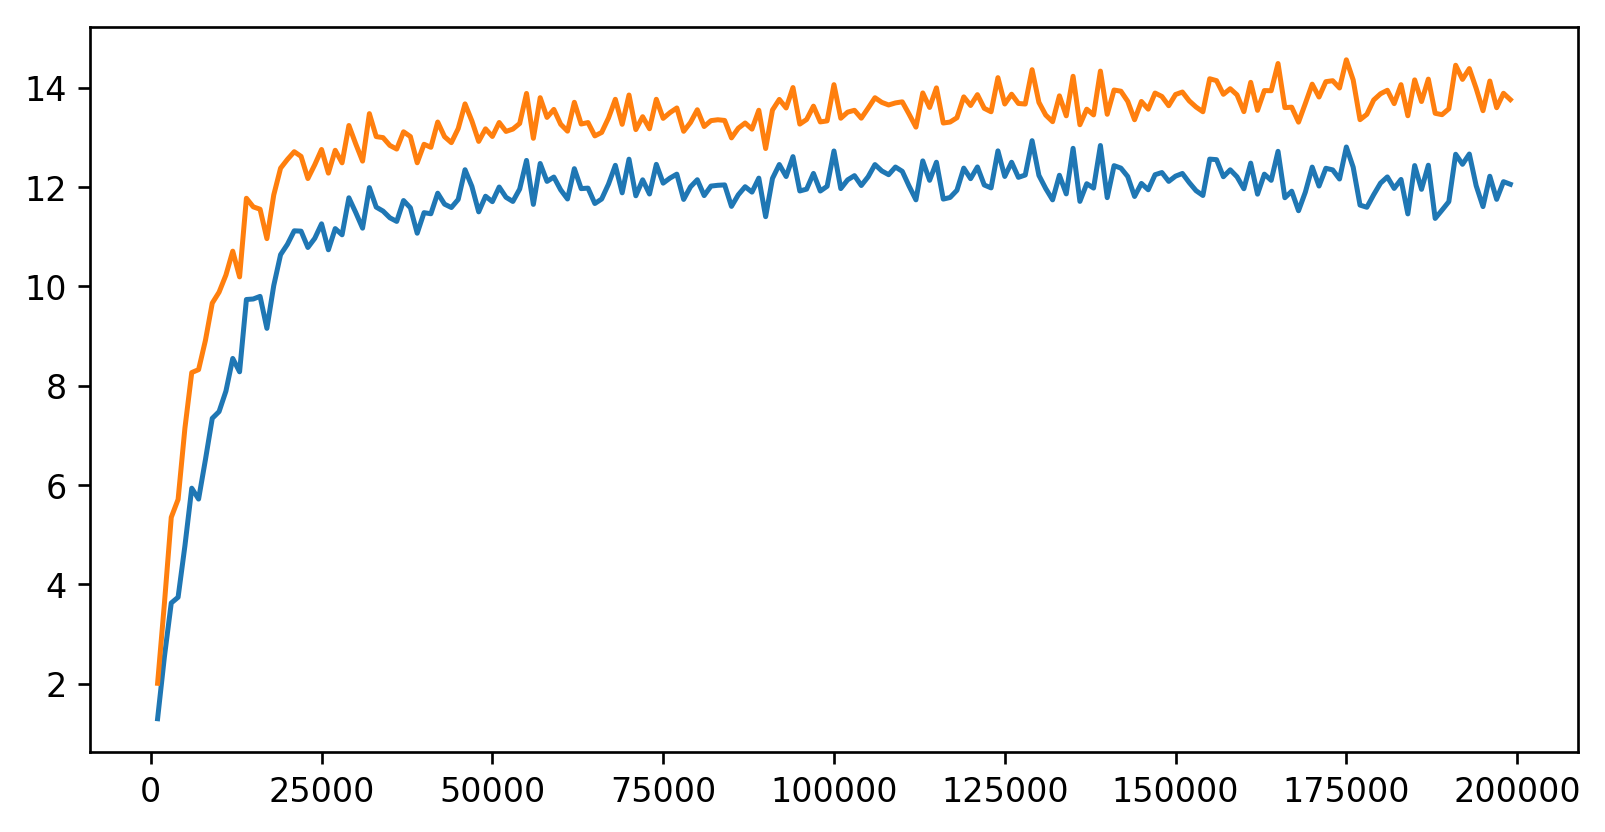
\includegraphics[width=0.9\linewidth]{figures/meanq.png}\hfill
  \caption{Mean Q-values of physician and agent actions}
  \label{fig:dqn_mean_q}
  \end{subfigure}
  \caption{Loss and mean Q-values of physician and agent actions for each epoch during the training phase.}
  \label{fig:dqn_train}
\end{figure}

\subsection{Restricting Actions}

Following the discretization suggested by \cite{DBLP:journals/corr/RaghuKCSG17}, we used 750 states and 25 discrete actions.
This led to a large space for all possible $s, a, s'$ transitions ($750 \times 25 \times 750$). 
As shown in Figure \ref{fig:transition-space}, observed transitions were at least two orders of magnitude
less frequent than possible transitions. Furthermore, observed transitions with sufficient 
samples ($n > 30$) were another order of magnitude smaller. Finally, there were certain
observed transitions that did not have sufficient data in order to determine if a given
physician action was effective. The area where there were sufficient examples but no physician consensus 
was deemed as the ideal exploration space for our mixture of experts. The percentage of physician 
consensus of a given action over all observed actions was a tunable hyperparameter used in our subsequent models.

\begin{figure}[H]
  \centering
  \begin{subfigure}{0.45\linewidth}
  \centering
  	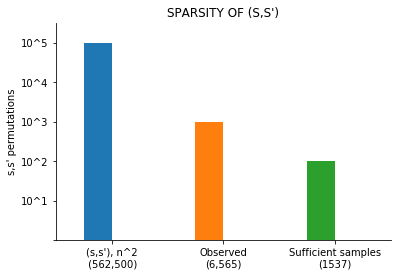
\includegraphics[width=1.0\linewidth]{figures/s-s_sparsity.png} %\hfill
  	\caption{$s, s'$ sparsity}
  	\label{fig:s-s_sparsity}
  \end{subfigure}%
  \begin{subfigure}{0.55\linewidth}
  \centering
  	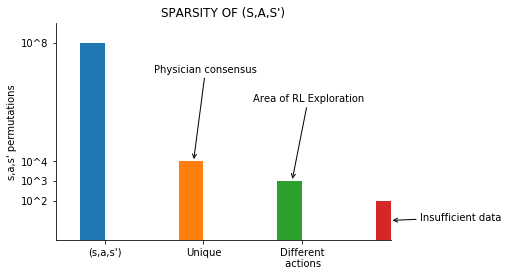
\includegraphics[width=1.0\linewidth]{figures/s-a-s_sparsity.png}\hfill
  	\caption{$s, a, s'$ sparsity}
  	\label{fig:s-a-s_sparsity}
  \end{subfigure}
  \caption{Sparsity of transition space}
  \label{fig:transition-space}
\end{figure}


\subsection{Mixture-of-Experts}

According to \cite{parbhoo2017combining}'s work, due to the heterogeneity of the patient dataset, it is difficult for one single model to perform well on all types of patients. Therefore, we consider combining the kernel policy as well as the DQN policy with the hope of further improving the treatment. For any given patient, our kernel expert is able to find a similar patient group, such that the derived policy works optimally for such type of patient. If the patient type is atypical, our DQN expert can effectively suggest action based on patient's continuous state representation. Thus, by taking advantage of their differing strengths, we build the mixture-of-experts model. We attempted two approaches to combine kernel and DQN experts, we call the first approach logistic-based switching. It utilizes logits to decide at any given state, taking which expert action would maximize the objective. We call the second approach RL-based gating, which applies a tree-based searching algorithm to pick actions that minimize the mortality rate.

\subsubsection{Logistic-based Switching}

In order to select the appropriate therapy combination, our mixture-of-experts takes the following inputs: kernel policy, DQD policy trajectory length, distance between a patient and its distance with 500th neighbor, age, gender and weight. We use WDR (weighted double robust estimator)\cite{thomas2016data}, which is the unbiased evaluation of the learned policies, as the objective function, and update the weights using gradient ascent via Autograd \cite{maclaurin2015autograd}

\begin{align}
\label{func:wdr}
WDR(D) := \sum_{i=1}^n\sum_{t=0}^{\infty} \gamma^tw_i^tR_t^{H_i} -  \sum_{i=1}^n\sum_{t=0}^{\infty}\gamma^t(w_t^i\hat{q}^{\pi_e}(S_t^{H_i}, A_t^{H_i}) - w_{t-1}^i\hat{v}^{\pi_e}(S_t^{H_i}))
\end{align}

Evaluation policy is computed as follows: 
\begin{enumerate}
\item Compute probability of taking Kernel action and DQN action as $p_{K} = logit(h(\mathbf{x}_t^{H_i})),\,\,p_{D} = 1- p_{K}$. 
\item One hot encode Kernel action and DQN action as $A_K^{25}$ and $D_K^{25}$; 
\item Combine Kernel policy and DQN policy as $\pi(S_t^{H_i}) = p_{K}A_K + p_{D}A_D$.
\end{enumerate}

In our reward formulation described in section \ref{section:reward_formulation}, the reward signals are sparse. This sparsity may cause the instability of the WDR estimator. To stabilize the estimator, intermediate rewards, i.e. a non-zero reward issued in non-final state, are needed. Since the value function and $Q$ function in equation \ref{func:wdr} are meant for reducing variance, it is not necessary to be accurate. Therefore, we build MDP models based on training data and compute the $V$ and $Q$ functions via an approximation.  

\subsubsection{RL-based Gating}

We also attempted a novel solution for MoE gating, namely using a reinforcement learning approach. We examined the literature but found little to no
information about previous attempts to use RL as MoE gating function. We used a tree-search
in this iteration. A future iteration could flatten the tree into a $Q$ function.

In this scenario, there are effectively three experts: the set of physicians, the kernel and the DQN. Each
expert suggests an action. The action with the highest reward is performed. The search continues
until the best action leads to patient mortality or the maximum search depth is reached at which 
point the patient is presumed to survive.

\begin{algorithm}
\caption{RL MoE - Tree Search Algorithm}\label{euclid}
\begin{algorithmic}[1]
\Procedure{ChooseAction}{}
\While {$depth < maxDepth$}
	\If {$\textit{physicianConsensus(state)} > \textit{threshold}$}
    	\State {$action \gets physicianAction$}
    \Else
    	\ForAll{experts}
          \State {$expertAction \gets \max( value(state))$}
        \EndFor
        \State {$action \gets \max(expertAction)$}
    \EndIf
    \State {$reward, state \gets \text{perform}(action)$}
    \If {$reward < 0$}
    	\State {$died \gets $} \textbf{true}
        \State break
    \EndIf
    \State {$depth \gets depth + 1$}
\EndWhile
\EndProcedure
\end{algorithmic}
\end{algorithm}

If there was a significant physician consensus to perform a given action in a given state, 
we bypassed the mixture-of-experts and selected the quorum action. The logic here is that 
if sufficient physicians are performing a given action, then that action is deemed to be trustworthy. 
The quorum threshold was a hyperparameter that afford easy tuning depending on confidence
in physician choices. 

This hyperparameter had a significant impact on the resulting
policy. If the consensus threshold was set too low, the most common physician action was taken 
all the time, leaving no opportunity for the algorithmic experts to find a better path among
the alternative physician choices. If the physician threshold was set too high, the physician
action was rarely taken and the algorithms would attempt to find an action that incredulously
led to zero mortality. After many iterations of hyperparameter tuning, we determined that physicians
needed to agree on
a given action 20\% of the time as the best balance. Note that this value may change significantly
if the semantic definition of action and state is modified.

Given the lack of reliable intermediate rewards, we attempted a very simple reward function
that empirically worked well. We examined the terminal state for all episodes. The results were
distributed with no apparent pattern. We then summed up the rewards found at the terminal 
state ($\pm 15$) and divided the by the frequency of the state occurring terminally. 
The result is in figure \ref{fig:expected_reward} which shows a useful signal. Further 
investigation into the merits of this approach is discussed in Section \ref{RLreward}.

\begin{figure}[H]
  \centering
  \begin{subfigure}{0.5\linewidth}
  \centering
  	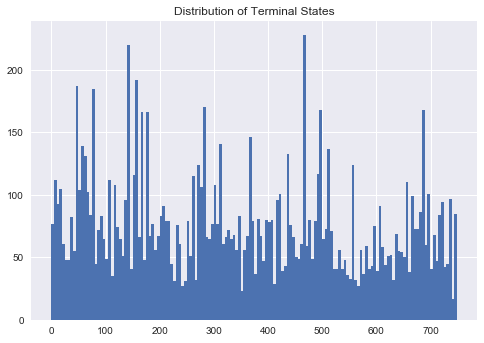
\includegraphics[width=1.0\linewidth]{figures/reward_by_state.png} %\hfill
  	\caption{Distribution of Terminal States}
  \end{subfigure}%
  \begin{subfigure}{0.5\linewidth}
  \centering
  	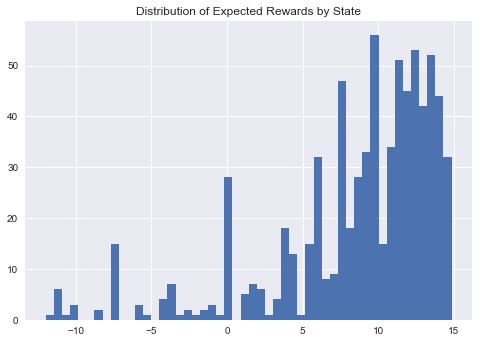
\includegraphics[width=1.0\linewidth]{figures/expected_reward.png}\hfill
  	\caption{Distribution of Calculated Reward by State}
	\label{fig:expected_reward}
  \end{subfigure}
  \caption{RL MoE - Reward Function}
\end{figure}

% \begin{figure}[H]
%   \centering
%   \begin{subfigure}{0.5\linewidth}
%   \centering
%   	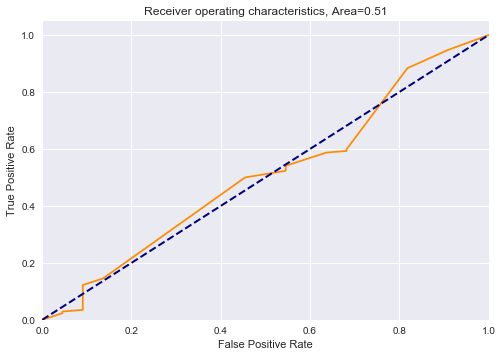
\includegraphics[width=1.0\linewidth]{figures/ROC.png} %\hfill
%   	\caption{ROC for Sigmoid of Expected Rewards}
%   	\label{fig:RL-ROC}
%   \end{subfigure}%
%   \begin{subfigure}{0.5\linewidth}
%   \centering
%   	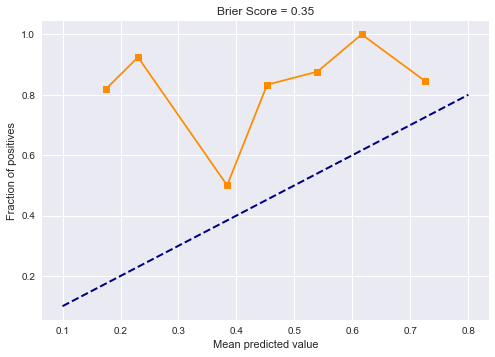
\includegraphics[width=1.0\linewidth]{figures/brier.png}\hfill
%   	\caption{Brier Calibration}
%   	\label{fig:RL-brier}
%   \end{subfigure}
%   \caption{Evaluation of RL Reward}
%   \label{fig:rl-reward}
% \end{figure}

\section{Policy Evaluation}

We now focus on the evaluation of our policies using the test data set.

\subsection{Logit Mixture-of-experts}
\label{section:dqn_policy}
We first show the action distributions over the test set under physician, kernel expert, DQN expert, and mixture-of-experts policies. 

\begin{figure}[H]
  \centering
  %----------------
  \begin{subfigure}{0.5\linewidth}
  \centering
  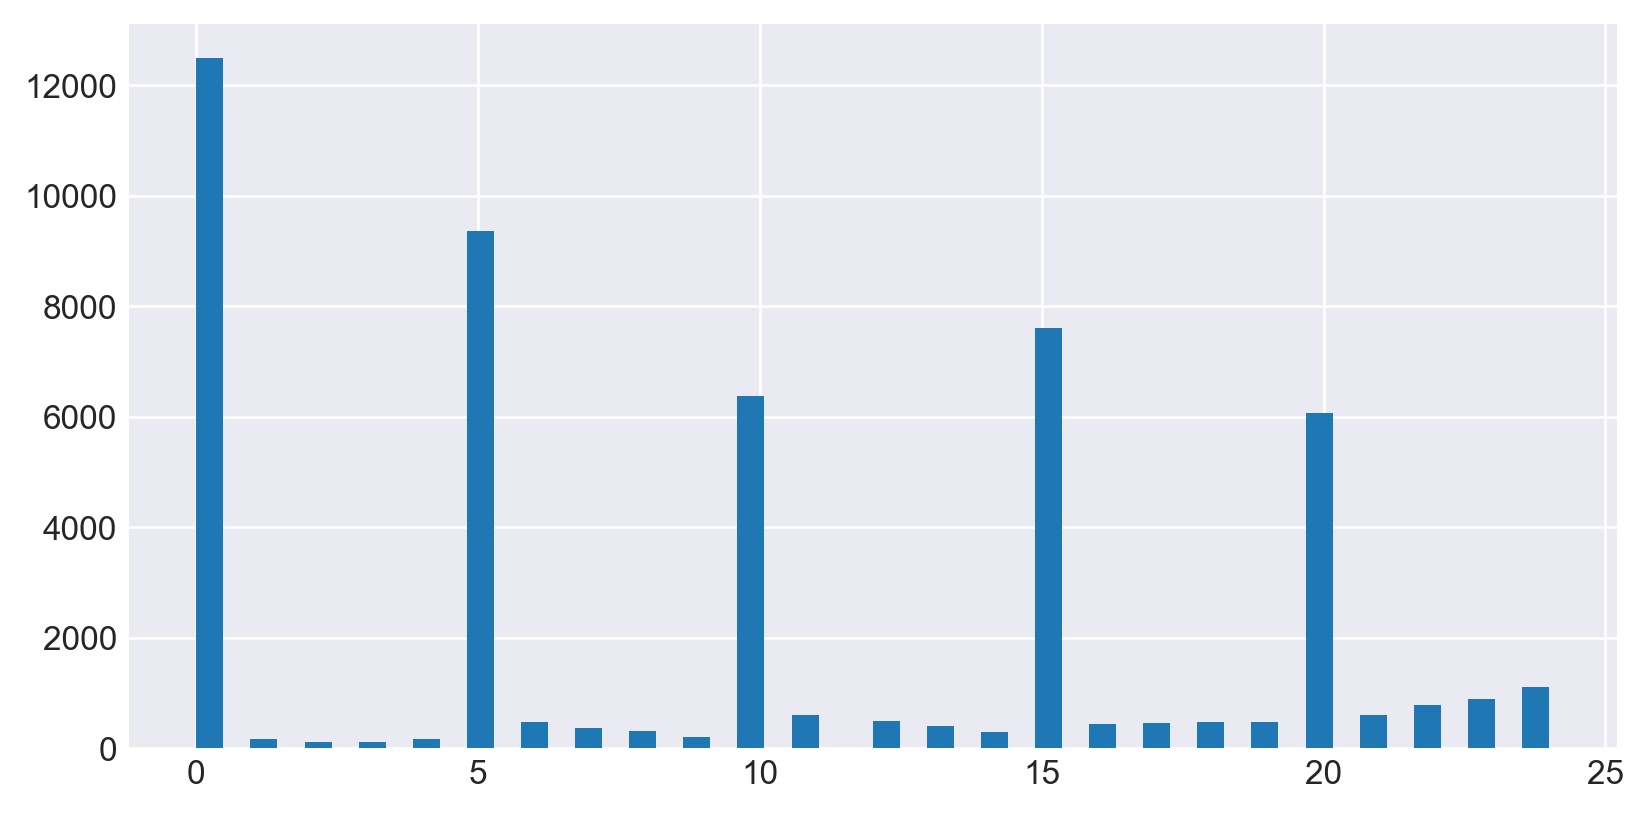
\includegraphics[width=0.9\linewidth]{figures/phy_test_a_hist.png}\hfill
  \caption{Physician action distribution over test set}
  \label{fig:phy_test_a_hist}
  \end{subfigure}%
 %------------------
  \begin{subfigure}{0.5\linewidth}
  \centering
  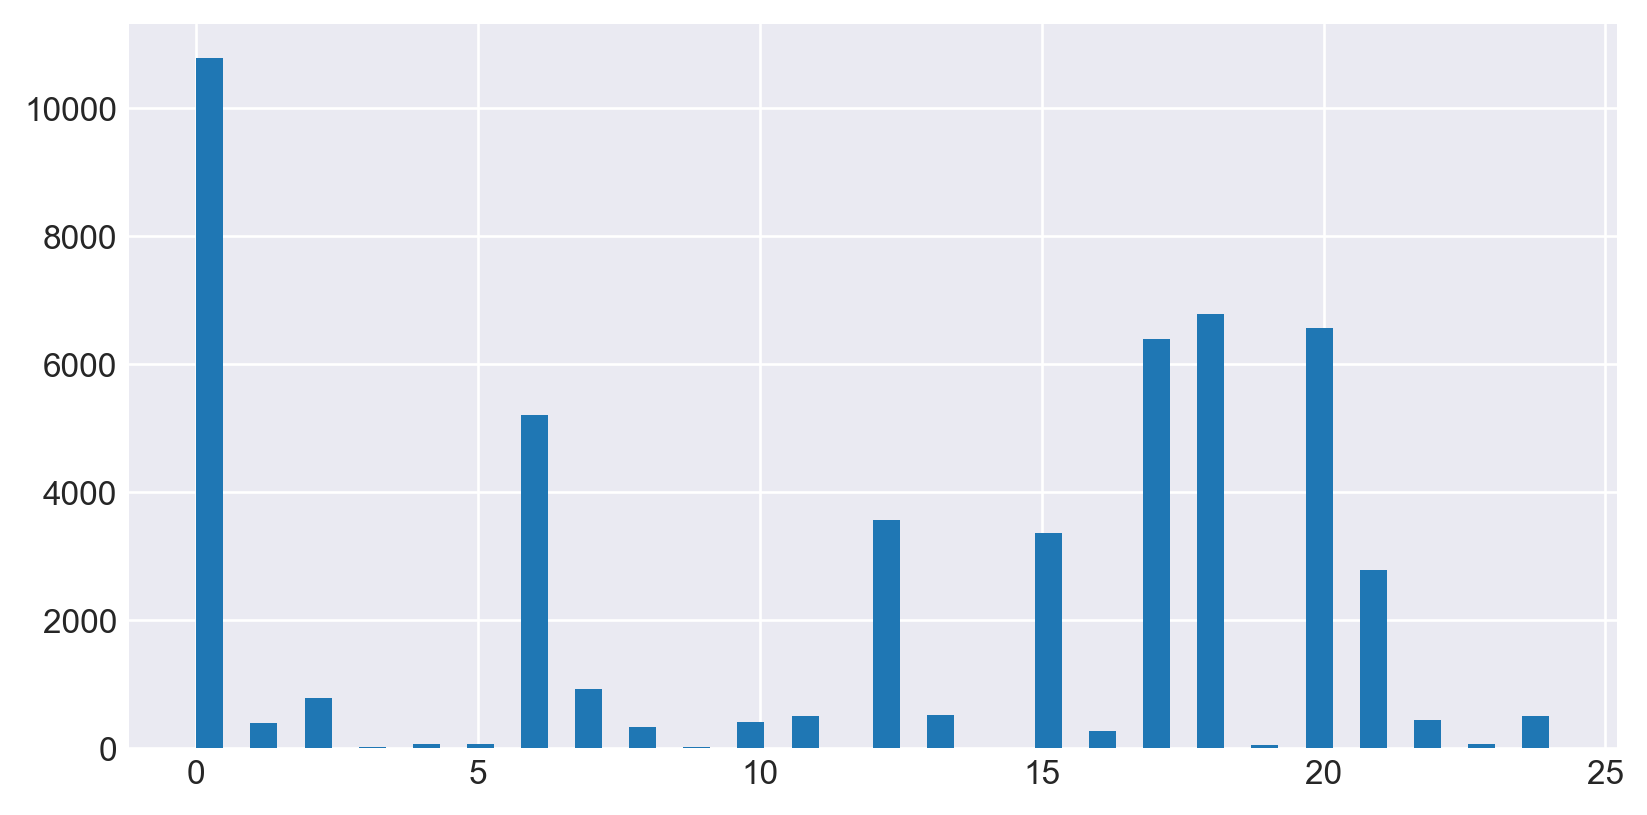
\includegraphics[width=0.9\linewidth]{figures/agent_test_a_hist.png}\hfill
  \caption{DQN action distribution over test set}
  \label{fig:agent_test_a_hist}
  \end{subfigure}
  %---------------
  \begin{subfigure}{0.48\linewidth}
  \centering
  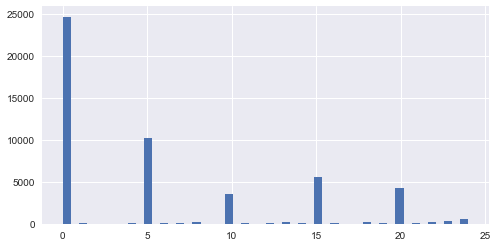
\includegraphics[width=0.9\linewidth]{figures/Kernel_test_bar.png}\hfill
  \caption{Kernel action distribution over test set}
  \label{fig:kenel_test_bar}
  \end{subfigure}
  %---------------
  \begin{subfigure}{0.48\linewidth}
  \centering
  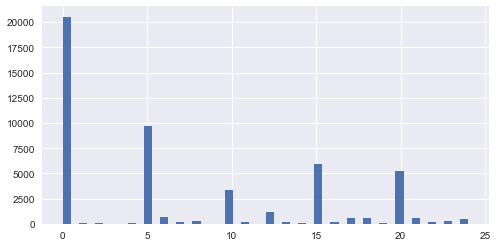
\includegraphics[width=0.9\linewidth]{figures/MOE_test_bar.png}\hfill
  \caption{MOE action distribution over test set}
  \label{fig:MOE_test_bar}
  \end{subfigure}
  %------------------
  \caption{Physician and agent action distributions over the test set}
  \label{fig:test_a_hist}
\end{figure}

\subsubsection{Action Distribution Comparisons}

As shown in Figure \ref{fig:test_a_hist}, 0, i.e. no treatment action, is dominant for all policies. In the following paragraphs, we compare the action distribution from our experts and physicians respectively. 

\textbf{Physician and DQN actions.}
Physician and DQN actions. Physician tends to prescribe actions 5, 10, 15, and 20 for patients with worse conditions. In terms of the agent, 6 instead of 5 and 12 instead 10 are prescribed more frequently. Both physicians and agent are in favor of 15. For actions beyond 15, physician only prescribe 20 frequently; however, besides 20, our DQN agent also tends to give more actions in this region, such as 17, 18, and 21.

\textbf{Physician and Kernel actions. }
Our kernel expert tends to be more conservative than the physician as it suggests no action approximately twice the   physicians' frequency. Actions which are in favored by physicians, such as 5, 10, 15, 20, are also prescribed often by the kernel expert. Our kernel expert action distribution shares the general behavior of a conservative physicians.

\textbf{Physician and Mixture-of-Experts actions. }
Over the test set, the mixture-of-experts select kernel action for over $87\%$ times; thus, the action distribution is similar to that of kernel expert. However, from \ref{fig:agent_test_a_hist} and \ref{fig:MOE_test_bar}, we can see that MOE prescribes more frequently actions 5, 10, 15, and 20. We can see that the mixture-of-experts is functioning
correctly as these actions are chosen by the DQN, not the kernel, expert. 

\subsubsection{IV and VP Dosage Comparisons}

We now examine how each expert prescribes iv-fluids and vasopressors. Figure \ref{fig:phy_test_action} shows that iv-fluids are largely used in the physician policy, and the usage as well as the dose volume of vasopressor is increased while higher dose of iv-fluids are given.

\begin{figure}[H]
  \centering
  \begin{subfigure}{0.5\linewidth}
  \centering
  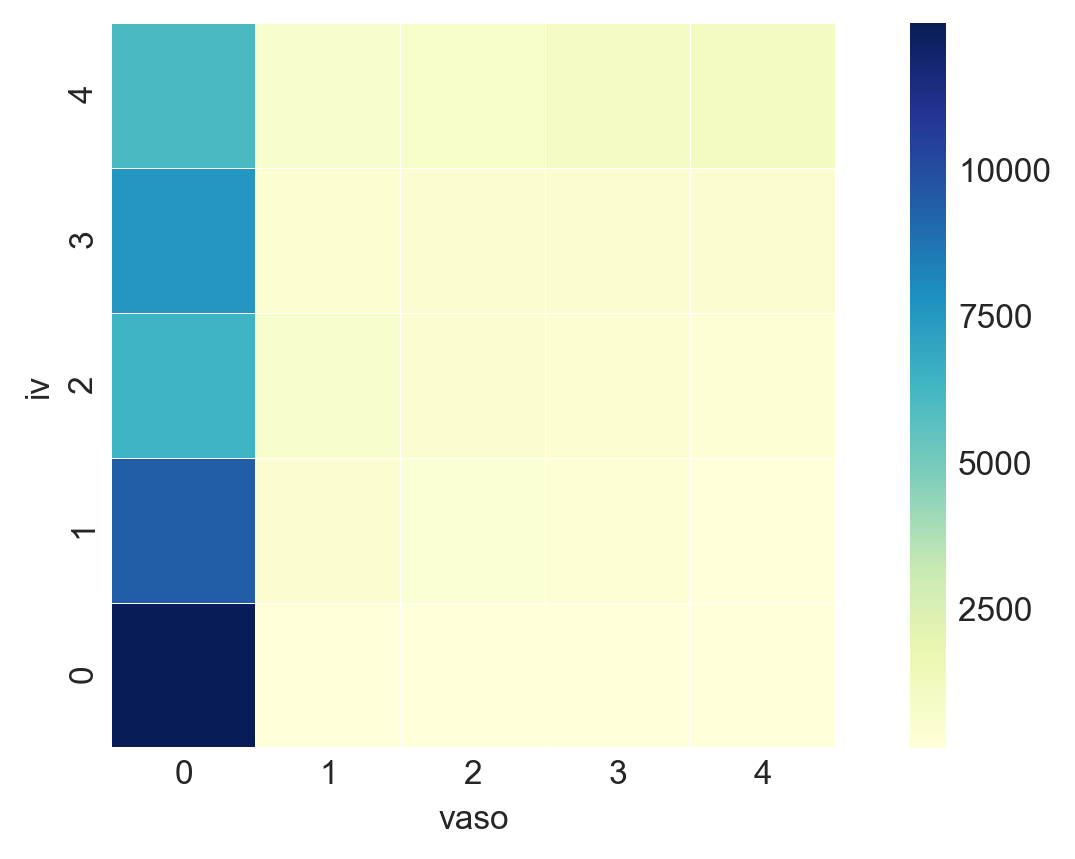
\includegraphics[width=0.9\linewidth]{figures/phy_test_actions.png}\hfill
  \caption{Physician action heatmap over test set}
  \label{fig:phy_test_action}
  \end{subfigure}%
  \begin{subfigure}{0.5\linewidth}
  \centering
  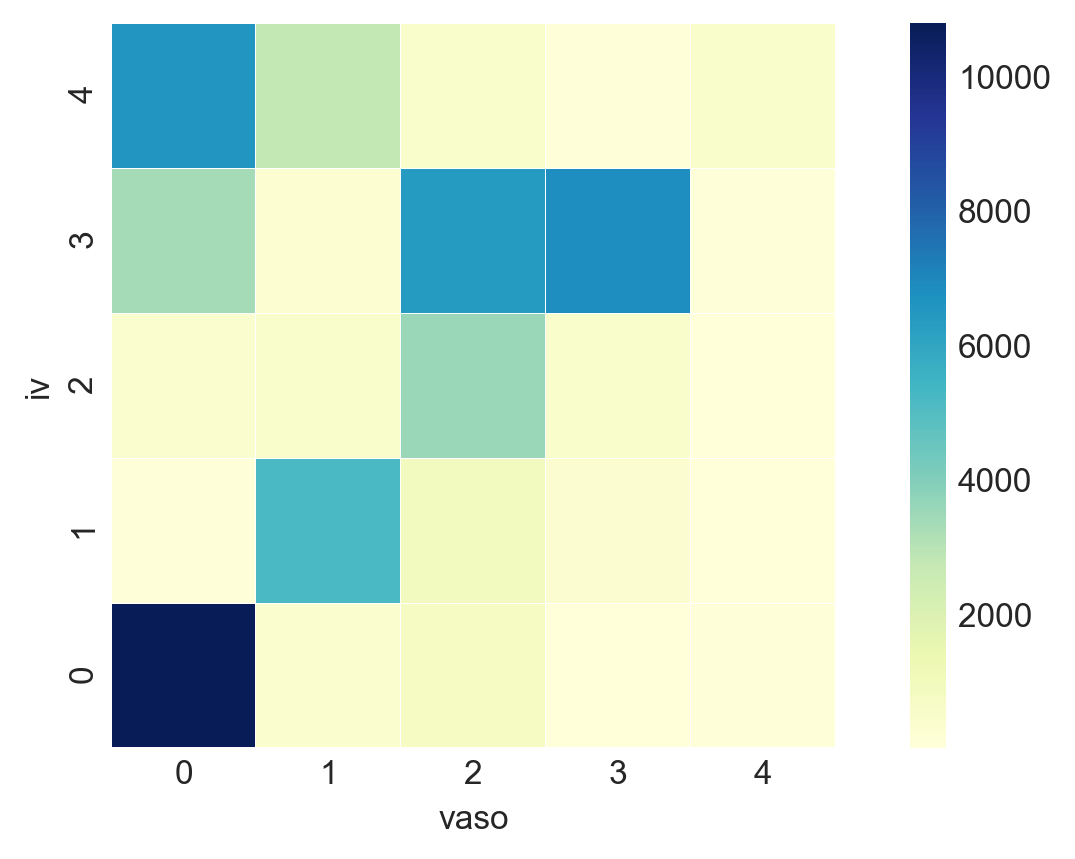
\includegraphics[width=0.9\linewidth]{figures/agent_test_actions.png}\hfill
  \caption{DQN action heatmap over test set}
  \label{fig:agent_test_action}
  \end{subfigure}
  \begin{subfigure}{0.48\linewidth}
  \centering
  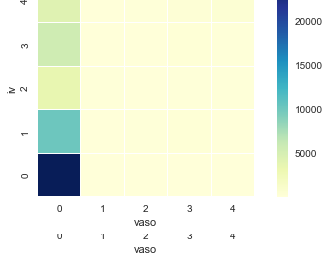
\includegraphics[width=0.9\linewidth]{figures/Kernel_test_heatmap.png}\hfill
  \caption{Kernel action heatmap over test set}
  \label{fig:Kernel_test_heatmap}
  \end{subfigure}
  \begin{subfigure}{0.48\linewidth}
  \centering
  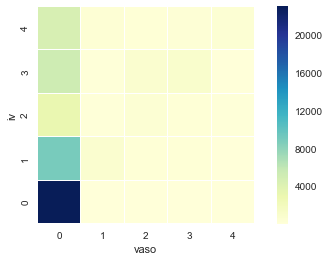
\includegraphics[width=0.9\linewidth]{figures/MOE_test_heatmap.png}\hfill
  \caption{MOE action heatmap over test set}
  \label{fig:MOE_test_heatmap}
  \end{subfigure}
  \caption{Physician and agent action heatmap over the test set}
  \label{fig:test_action_heat}
\end{figure}

With respect to the DQN policy, this tendency becomes more obvious. Note that in Figure \ref{fig:agent_test_action}, the actions represented by these diagonal cells are used more often than in physician policy. However, just like the physician, the agent is scrupulous about prescribing the maximum dose of vasopressor. In general, the agent is suggesting that the iv-fluids and vasopressor should be prescribed comparatively more frequently. Kernel policy is close to the physician policy except it is even more conservative in giving high dosages for both IV-fluids and vasopressor. Finally, since the kernel actions are chosen $7$ times more often than DQN actions, the mixture-of-experts acts much akin to the kernel expert. However, we do can observe that in \ref{fig:MOE_test_heatmap}, the diagonal cells appear deeper, implying that the MoE chooses the action suggested by the DQN experts that for patient under certain physiological states where higher dosages of vasopressor is required.

\subsubsection{Off-policy Evaluation using WDR}

We run WDR on policies suggested from physician, kernel, DQN, and MOE. Table \ref{table:WDR_estimate} shows that over both training and testing sets, mixture-of-experts policy achieves the highest unbiased estimation.


\begin{table}[H]
\caption{\label{table:WDR_estimate}WDR estimate for different policies}
\centering
\begin{tabular}{|l|r|r|}
\hline
Policy & Train & Test \\ \hline
Physician & 6.89 & 7.13 \\ 
DQN & 8.09 & 8.65 \\ 
Kernel & 9.35 & 4.59 \\ 
Mixture of Expert & 11.16 & 8.81 \\
\hline
\end{tabular}
\end{table}

\subsubsection{Logistic Switching Weight Interpretation}
To enable the mixture-of-experts to switch actions, we need to assign a probability distribution over actions from experts based on a given patient's features. For each patient, the features we use are trajectory length (i.e. number of observations), furthest distance from its 500 nearest neighbors, age, gender, and weight.

% Figure shows the pre-trained weights for these features.

% \begin{figure}[H]
% \centering
% 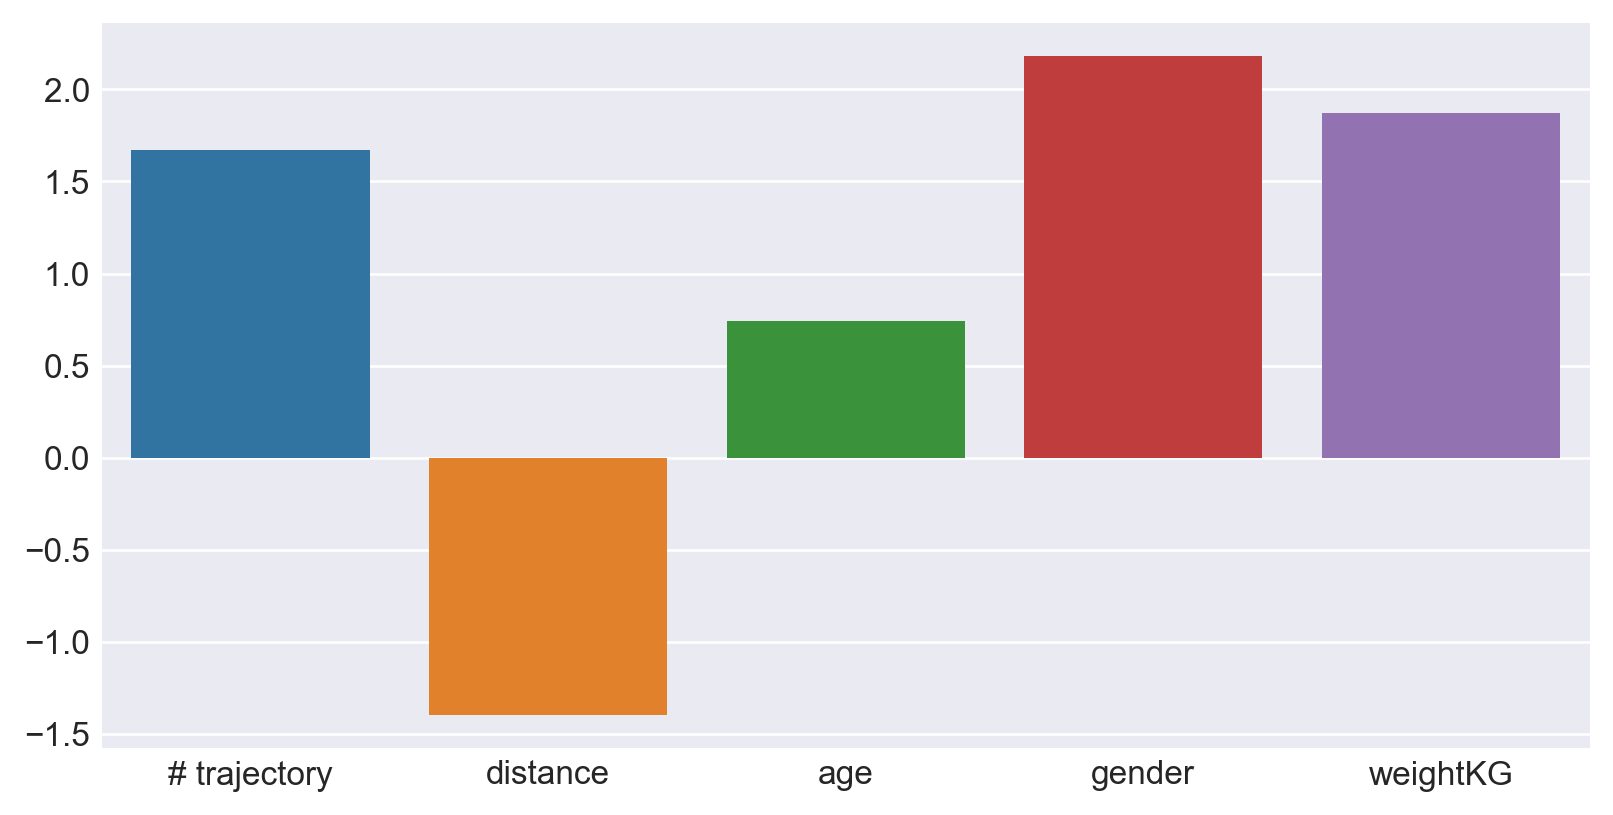
\includegraphics[width=0.4\textwidth]{figures/logstic_weights.png}
% \caption{\label{fig:logstic_weights} The pre-trained weights for patient features.}
% \end{figure}

After training, the weights for features are: trajectory length$=1.67$, max distance to neighbor $=-1.40$, age=0.74, gender=2.18, weight=1.87. As trajectory length increases, more patient information is available, which assists in finding reliable neighbor policies. Therefore, for longer trajectories, the logit prefers the Kernel action over the DQN action. In contrast, when the distance to the furthest neighbor is large, the Kernel policy will be unreliable, so the logit prefers DQN actions.

\subsection{RL Mixture-of-experts}

The resulting three expert mix provides a reasonable balance between a physician-only and an
algorithmic-only policy, especially when configured appropriately by the consensus hyperparameter. Using only 
two algorithmic experts (kernel, DQN), the resulting policy is more conservative than the 
logit-based gating function, favoring the kernel more frequently than the DQN.

\begin{figure}[H]
  \centering
  \begin{subfigure}{0.45\linewidth}
  \centering
  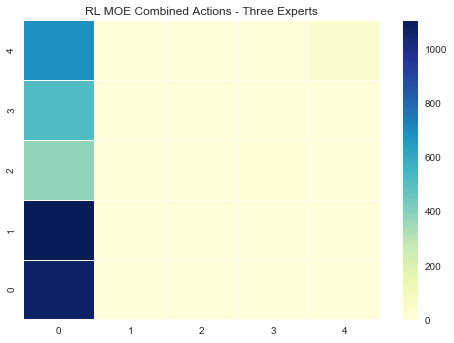
\includegraphics[width=0.9\linewidth]{figures/RLMOE3.png}\hfill
  \caption{RL MoE - Three Experts}
  \label{fig:RLMOE3}
  \end{subfigure}
  \begin{subfigure}{0.45\linewidth}
  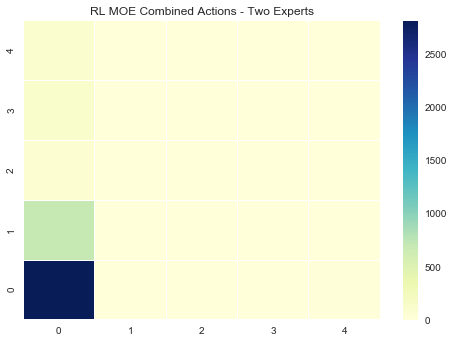
\includegraphics[width=0.9\linewidth]{figures/RLMOE2.png}\hfill
  \caption{RL MoE - Two Experts (Kernel, DQN)}
  \label{fig:RLMOE2}
  \end{subfigure}
  \caption{Resultant Policy from RL-based MoE}
  \label{fig:RLMOE}
\end{figure}

\begin{table}[H]
  \centering
  \caption{RL MoE Results - Three Experts}
  \begin{tabular}{|c|c|c|}
    \hline
     Physician Consensus & Est. Mortality & Consensus Occurred \\
     \hline
    10\%  & 13.4\% & 100.0\% \\
    \hline
    20\% & 10.0\% & 23.1\%\\
    \hline
  \end{tabular}
\end{table}


Examining the frequency of consensus between the different experts was enlightening as the
algorithmic approaches agreed more frequently than the physician chosen action. Investigating 
this discrepancy is a potential area of further research.

\begin{table}[H]
  \centering
  \caption{Action Agreement Frequency - Three Experts}

  \begin{tabular}{|l|c|c|}
    \hline
      & Kernel & DQN\\
     \hline
    Physician  & 4.1\% & 3.3\% \\
    \hline
    Kernel & & 45.4\% \\
    \hline
  \end{tabular}
\end{table}

\textbf{By using the MoE (including accounting for physician policy), we project a significant improvement in patient mortality (13.4\% vs. 10.0\%).} This appears very promising so caveats are discussed in the sections below.


\section{Limitations}

\subsection{Use of WDR as Logit Gradient Function}
As the authors of WDR acknowledge in a subsequent paper\cite{liumodel}, WDR is prone to instability:

\blockquote{
Recent work such as doubly robust and MAGIC, shows that we can get benefit from combining importance sampling method with model value.
However they all assume that they have only one model. In case we have several different models, which is common
in some complex domains, it may be hard to select the best one from them, and may lose the potential benefit from
all models. we present a evidence example to show that select model by simply minimizing the notation of error in
previous estimator (MAGIC) can fall into a wrong model, which suggest that selecting a best model for off-policy policy
evaluation is non-trivial and worth of further exploration. } 

WDR furthermore requires an intermediate reward function, which was not readily available in the 
dataset. We iterated through numerous rounds of feature engineering in attempting to 
find an intermediate reward that had reasonable predictive value, ultimately choosing change
in SOFA score and change in Arterial Lactate over a single period. 
(See Appendix \ref{appendixintermediate} for a discussion of our intermediate reward
investigation).

\subsection{Intermediate Rewards}
Our MoE approach, using both conventional gradient gating as well as an RL-based approach
were stymied by the lack of high quality value function or intermediate rewards. As we have seen numerous
times in other research, RL success hinges on having
a stable and predictive value function. Once the value function is reliable, the
policy iteration becomes significantly easier. Without a reliable value function, 
policy iteration is impossible. This is analogous to neural net-based supervised learning:
without a quality training set, a supervised learning algorithm cannot perform well.
Intuitively, a better intermediate reward function and a better loss function would yield
even more promising results from a mixture-of-experts.


\subsection{RL MoE Reward Function}
\label{RLreward}
While the results of the RL-based MoE appear encouraging, and the resulting policy seems
reasonable, it is recommended to perform a more thorough evaluation of the 
predictability of the expected reward metric. An ROC analysis and a Brier Calibration test would
give greater credibility to this reward function and the RL-based MoE in general.

\subsection{RL MoE has Markov and Deterministic Assumptions}

The RL MoE makes two assumptions: that the state transitions are Markov, which may
not be the case. We also assume that actions are deterministic, where a given action
will always lead to a given new state. A future version would relax this assumption
by modeling stochasticity based on the known distribution of $s, a, s'$ from the
training set. Modeling stochasticity would also be a more realistic means of measuring mortality.

\section{Discussion}

As shown in figure \ref{fig:test_action_heat}, each expert has different behaviors. 
The kernel method is most conservative, tempering variance of different physician
actions. The DQN has higher variance which leads to more aggressive actions for
patients that may need more intervention earlier. The overall combination
yields a generally conservative approach. The heatmaps occlude the cases where
DQN has found a better treatment course for patients that are outliers. Given the small
number of patients in this category, the DQN is an appropriate means of finding 
appropriate pathways that are outside the capabilities of the conservative kernel method.
Per our original objective, treatment has become more personalized.

Perhaps in combination with
another team using Inverse Reinforcement Learning, it would be possible to find an 
appropriate reward function to drive both the WDR and the RL based gating functions.

Even with the very simplistic reward function, the experimentation with RL-based 
gating yielded several interesting ideas worth pursuing. The specific questions raised include:

\begin{itemize}
\item Could the human specialist (physician in this case) be considered simply another
expert in the mixture? What priority should physician actions be given over algorithmic
suggestions? Examining
where disagreements occur between human and between algorithms may yield interesting
insight into the decision making process for both approaches.
\item Assuming a viable reward function exists, is it possible to simply evaluate all
observed physician actions and choose the policy based on which patients are receiving
the reward (ie. lower mortality in this case) more frequently? In other words, 
especially in the case of medicine, what kind of policy choices can be offered to the
physician at the moment of decision making that provide useful, reliable information regarding
interventions made by peers in similar circumstances?
\end{itemize}


\section{Future Work}

Creating a robust simulation environment is highly desirable in order to ascertain the effectiveness
of novel treatment strategies. While there has been some efforts in using Recurrent Conditional GANs for generation of sepsis training data \cite{esteban2017real}, a model-based approach is possibly less 
prone to the instability often found in GANs. If a physiological model is difficult due to lack of 
domain knowledge, an alternative data-driven approach may be the use of 
microsimulation, which has been previously used in sepsis and ICU treatment evaluation although not in an
RL context
\cite{clermont2004dynamic,saka2007use}.

The use of restricted actions based on observed physician actions would be interesting to apply to other
treatment domains, even as a tool to evaluate consistency of treatment. This could also be used as a means
of determining more precisely which interventions led to lower mortality. Finally, it may
serve a useful as a clinical tool for physicians to consult before performing interventions, answering
questions such as: ``What did other physicians do for patients in this state? With what frequency? What was the 
mortality?''

The idea of using an RL-based MoE gating function, especially in problems that lend themselves
to an RL approach (as opposed to a differentiable loss function) is worth investigating.
One recent paper \cite{shazeer2017outrageously} from Google Brain (Hinton, Dean, et al.) alludes
to this but offers no specifics as to a means of policy iteration. 

The area of off-policy policy evaluation merits further investigation, especially in cases
where only replay of past history is available. A robust mechanism would open RL to a much
larger set of problem spaces while potentially offering higher safety by minimizing risky explorations.
The high variance of current approaches leave room for significant improvement.

As mentioned previously, a more rigorous evaluation of the RL-based reward function
would be desirable to ensure the credibility of this approach.

\section{Conclusion}

Sepsis management is an interesting and engaging problem space, with potential for
significant human impact. We ambitiously attempted several approaches, some of which were
novel. We feel there are interesting areas meriting further exploration, both from a sepsis
treatment standpoint as well from a general machine learning approach. Initial results 
are promising showing a significant decrease in projected patient mortality. Combining human
and algorithmic policies in domains with high consequences such as healthcare can lead
to both better, more specific policies that are potentially safer and more effective
than current practices.

\section*{Acknowledgements}

We would like to express our sincere gratitude to Prof. Doshi-Velez, Dr. Matthieu Komorowski
and Omer Gottesman for their
advice, guidance and candid questioning of the approaches we attempted. We especially appreciate their
patience as this project changed direction and emphasis. We would also like to thank the other
students in Harvard CS282R Fall 2017 for their insights, encouragement and feedback.

\newpage
\begin{appendices}

\section{Simulation Environment for RL}

Given the sample inefficiency of training a DDQN, we initially evaluated creating a simulator
of a patient's clinical course. This would have allowed experimentation with novel treatments
for which there was no empirical data. Simulation has been used successfully in many RL 
scenarios, most visibly in the use of the Atari simulation 
environment \cite{DBLP:journals/corr/abs-1207-4708} for the creation of DQNs \cite{DBLP:journals/corr/MnihKSGAWR13} 
/ DDQNs \cite{wang2015dueling}.

Unfortunately, the model-based Sepsis simulators available today (for example \cite{breuer2004intensive}) are used primarily for physician
training and are not appropriate for use as an RL training environment. 

We did attempt to create synthetic data by mimicking the observation distributions found in the source
data set. However, we abandoned this effort because we felt that it would not be providing a robust
representation of novel interventions since there was no supporting data and may suffer from biases.
The analysis of the state distributions did prove useful for restricting actions.

\section{Intermediate Reward Investigation}
\label{appendixintermediate}
In order to determine an intermediate reward function, we explored several options. 

\subsection{Observations Correlated with Mortality}

Performing a correlation yielded the following most correlated observations:
\begin{table}[H]
\caption{Observations Most Closely Correlated with 90 Day Mortality}
\centering
\begin{tabular}{|l|c|}
\hline
Observation & Correlation \\ \hline
SOFA & 0.25 \\ 
BUN & 0.23 \\ 
age & 0.21 \\ 
Elixhauser & 0.16 \\
SIRS & 0.15 \\
\hline
\end{tabular}
\end{table}

\subsection{Classification Results}

We then attempted a variety of classifiers using the above features and measured the F1 score. 
We also evaluated accuracy against a larger set of features. The accuracy of multiple classifiers
did not sufficiently exceed the baseline.
The following table summarizes the results for the best F1 score and the relevant hyperparameter.

\begin{table}[H]
\label{table:classifier}
\caption{Classification Performance on Training Set}
\centering
\begin{tabular}{|l|l|c|c|}
\hline
Classifier & Hyperparameter & F1 Score & Accuracy \\ \hline
Baseline & N/A & N/A & 0.77 \\
Logisitic Regression & $C=0.1$ & 0.07 & 0.79 \\ 
Random Forest & Trees $= 100$  & 0.33 & 0.78 \\ 
kNN & $k=10$ & 0.29 & 0.77 \\ 
SVM & $C=0.0001$ & 0.07 & 0.77\\
XGradBoost & estimators$=200$ & 0.30 & 0.79 \\
\hline
\end{tabular}
\end{table}

Given the low correlation, low F1 score, and baseline accuracy, we did not see strong
predictive value for mortality in the observations.


\end{appendices}


\bibliographystyle{alpha}
\bibliography{sample}

\end{document}